%!TEX root = ../BUSystematics.tex

\graphicspath{{Body/Figures/Pileup/}{Body/Figures/Pileup/Amplitude/}{Body/Figures/Pileup/TimeShift/}{Body/Figures/Pileup/EnergyModel/}{Body/Figures/Pileup/TriplePileup/}{Body/Figures/Pileup/RateError/}}

\section{Pileup Systematic Uncertainties}


- describe generality of pileup correction here, don't go into too much detail on it though
- I use ``I'' throughout the text a lot here, I need to change all of that



         \begin{gather}
            E_{\text{doublet}} = C \cdot (E_{\rm T} + E_{\rm S}), \label{eq:Edoublet} \\
            t_{\text{doublet}} = \frac{t_{\rm T} \cdot E_{\rm T} + (t_{\rm S}-T_{G}) \cdot E_{\rm S}}{E_{\rm T} + E_{\rm S}} + \frac{T_{G}}{2}. \label{eq:tdoublet}
        \end{gather}



\subsection{Amplitude}

The pileup amplitude uncertainty is evaluated by applying a multiplier to the amplitude of the pileup correction and refitting. Multipliers were applied in steps of 0.01 from 0.9 to 1.1, and the resulting R vs pileup multiplier plot is fit to determine the sensitivity of \R to the pileup multiplier. The uncertainty in the multiplier is determined as the width of the parabola in the \chisq vs the pileup multiplier. The systematic uncertainty on \R is then calculated as 
    \begin{align}
        \delta R = \sigma_{P_{m}} \times \frac{dR}{dP_{m}},
    \end{align}
where $P_{m}$ is the value of the pileup multiplier. \figref{fig:PMscan} shows the scan results for the 9d dataset. \tabref{tab:pileupMultplierScan} show the scan results and \tabref{tab:systematicError_pileupMultplier} gives the systematic uncertainties for the Run~1 datasets.





\begin{table}[h]
\centering
% \setlength\tabcolsep{10pt}
\renewcommand{\arraystretch}{1.2}
\begin{tabularx}{0.9\linewidth}{XOOOO}
  \hline
    \multicolumn{5}{c}{\textbf{Pileup Amplitude Scan Results}} \\
  \hline\hline
    Dataset & \thead{Fit Method} & \multicolumn{1}{c}{$dR/dP_{m}$} & \multicolumn{1}{c}{$\sigma_{P_{m}}$} & \multicolumn{1}{c}{$P_{m_{\text{min}}}$} \\
  \hline
    \multirow{2}{*}{60h} & T & $-353.1$ & 0.061 & 0.981 \\
                         & R & $-308.3$ & 0.064 & 1.014 \\
  \hline
    \multirow{2}{*}{HighKick} & T & $-235.2$ & 0.049 & 0.981 \\
                              & R & $-217.0$ & 0.053 & 0.982 \\
  \hline
    \multirow{2}{*}{9d} & T & $-187.8$ & 0.043 & 0.988 \\
                        & R & $-217.6$ & 0.046 & 1.002 \\
  \hline
    \multirow{2}{*}{Endgame} & T & $-326.4$ & 0.031 & 0.879 \\
                             & R & $-269.0$ & 0.035 & 0.958 \\
  \hline
\end{tabularx}
\caption[]{Sensitivities, widths of \chisq plots, and minima of \chisq plots for the four Run~1 datasets and both fit methods. Units are either unitless or in ppb for the sensitivity.}
\label{tab:pileupMultplierScan}
\end{table}




\begin{table}[h]
\centering
\renewcommand{\arraystretch}{1.2}
\begin{tabularx}{0.65\linewidth}{XYY}
  \hline
    \multicolumn{3}{c}{\textbf{Systematic Uncertainties due to Pileup Amplitude}} \\
  \hline\hline
    Dataset & \thead{T-Method} & \thead{R-Method} \\
  \hline
    60h & 21.7 & 19.9 \\
    HighKick & 11.4 & 11.4 \\
    9d & 8.1 & 10.1 \\ 
    Endgame & 10.1 & 9.4 \\
  \hline
\end{tabularx}
\caption[]{Systematic uncertainty due to the pileup amplitude. Units are in ppb.}
\label{tab:systematicError_pileupMultplier}
\end{table}

\begin{figure}[h]
\centering
    \begin{subfigure}[t]{0.45\textwidth}
        \centering
        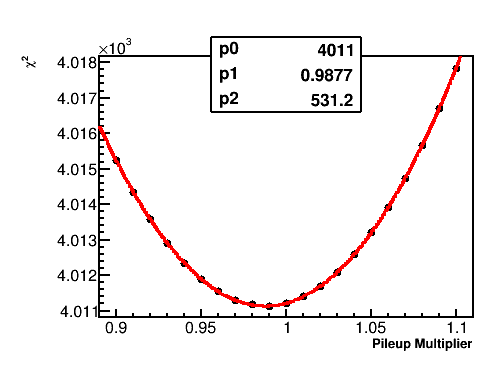
\includegraphics[width=\textwidth]{TMethod_Chi2_Vs_PileupMultiplier_Canv}
        \caption{T-Method \chisq versus pileup multiplier. The parabolic fit equation used was $y = p_{2}(x - p_{1})^{2} + p_{0}.$}
    \end{subfigure}% %you need this % here to add spacing between subfigures
    \hspace{1cm}
    \begin{subfigure}[t]{0.45\textwidth}
        \centering
        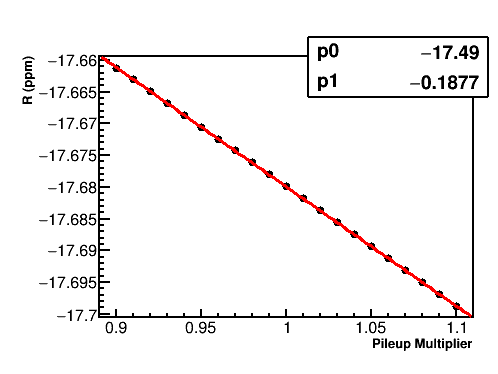
\includegraphics[width=\textwidth]{TMethod_R_Vs_PileupMultiplier_Canv}
        \caption{T-Method $R$ versus pileup multiplier. The parameter $p_{1}$ gives the sensitivity of $R$ to the value of the pileup multiplier, with units in ppm.}
    \end{subfigure}

    \begin{subfigure}[t]{0.45\textwidth}
        \centering
        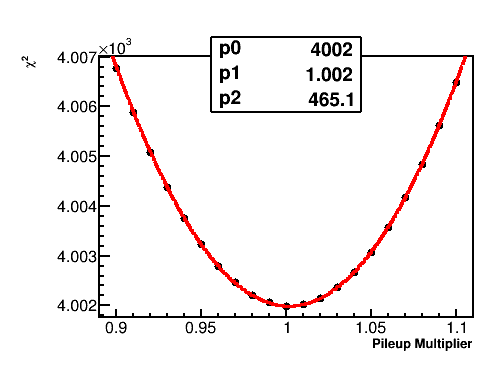
\includegraphics[width=\textwidth]{FullRatio_Chi2_Vs_PileupMultiplier_Canv}
        \caption{R-Method \chisq versus pileup multiplier. The parabolic fit equation used was $y = p_{2}(x - p_{1})^{2} + p_{0}.$}
    \end{subfigure}% %you need this % here to add spacing between subfigures
    \hspace{1cm}
    \begin{subfigure}[t]{0.45\textwidth}
        \centering
        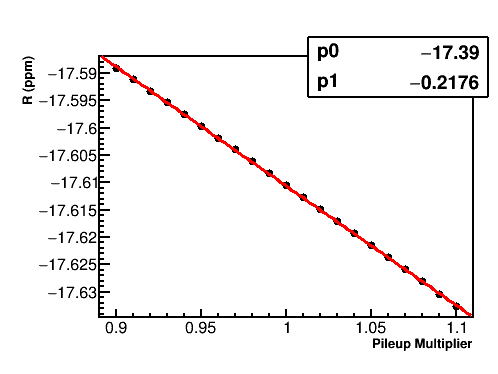
\includegraphics[width=\textwidth]{FullRatio_R_Vs_PileupMultiplier_Canv}
        \caption{R-Method $R$ versus pileup multiplier. The parameter $p_{1}$ gives the sensitivity of $R$ to the value of the pileup multiplier, with units in ppm.}
    \end{subfigure}
\caption[Pileup multiplier scan]{Pileup multiplier scan. Data are from the 9d dataset.}
\label{fig:PMscan}
\end{figure}



\clearpage
\subsection{Cluster Time Model}

The time of a constructed doublet in the pileup construction is set as the energy weighted time of the two singlets plus half the gap time. Previously the uncertainty was calculated by scanning over an additional time shift and then applying a conservative uncertainty of \ns{2.5}. The results of such a scan can be seen in \figref{fig:PTSscan}. If this procedure is used then the systematic uncertainty on \R is less than 15 ppb for all datasets.

That is however a pretty conservative approach. If I instead use the most energetic singlet time as the doublet time, then the $\Delta R$ is less than \ppb{1} for all datasets. If I instead set the doublet time as either the first singlet time, or the second singlet time, then the $\Delta R$'s are given in \tabref{tab:systematicError_clusterTimeDeltas} and range around 5-6~ppb. I take as my systematic uncertainty half this range for all datasets. The final systematic uncertainties are given in \tabref{tab:systematicError_clusterTimeModel}.



\begin{figure}[h]
\centering
    \begin{subfigure}[t]{0.45\textwidth}
        \centering
        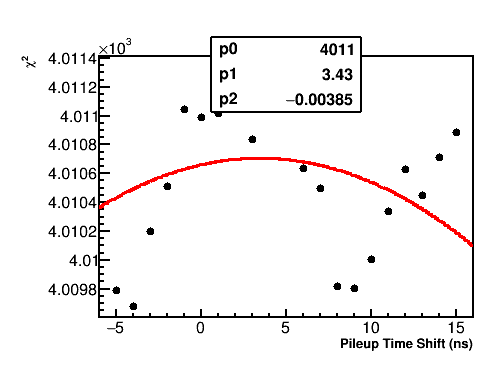
\includegraphics[width=\textwidth]{TMethod_Chi2_Vs_PileupTimeShift_Canv}
        \caption{T-Method \chisq versus pileup time shift. There is no clear minimum.}
    \end{subfigure}% %you need this % here to add spacing between subfigures
    \hspace{1cm}
    \begin{subfigure}[t]{0.45\textwidth}
        \centering
        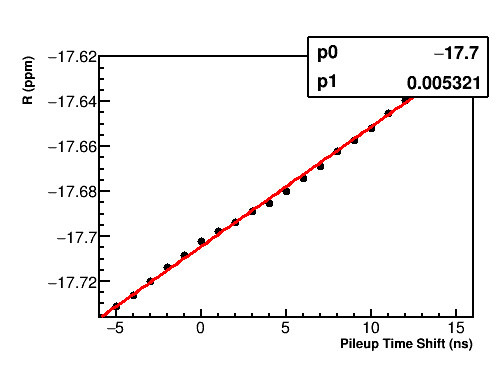
\includegraphics[width=\textwidth]{TMethod_R_Vs_PileupTimeShift_Canv}
        \caption{T-Method $R$ versus pileup time shift. The parameter $p_{1}$ gives the sensitivity of $R$ to the value of the pileup time shift, with units in ppm.}
    \end{subfigure}
\caption[Pileup time shift scan]{Pileup time shift scan for the T-Method. The R-Method plots look the same. Data are from the 9d dataset.}
\label{fig:PTSscan}
\end{figure}


\begin{table}[h]
\centering
\renewcommand{\arraystretch}{1.2}
\begin{tabularx}{0.85\linewidth}{@{\extracolsep{\fill}}XYY|YY}
  \hline
    \multicolumn{5}{c}{$\Delta R$ with first and last singlet times} \\
  \hline\hline
            & \multicolumn{2}{c|}{T-Method} & \multicolumn{2}{c}{R-Method } \\
    Dataset & \thead{First Time} & \multicolumn{1}{c|}{Last Time} & \thead{First Time} & \thead{Last Time}  \\
  \hline
    60h & -5.5 & 4.6 & -8.0 & 4.8 \\
    HighKick & -5.0 & 4.3 & -5.6 & 4.0 \\
    9d & -5.4 & 5.6 & -5.8 & 5.4 \\ 
    Endgame & -4.5 & 4.4 & -5.2 & 4.3 \\
  \hline
\end{tabularx}
\caption[]{$\Delta R$ when applying the two singlet times as the doublet times. Units are in ppb.}
\label{tab:systematicError_clusterTimeDeltas}
\end{table}



\begin{table}[h]
\centering
\renewcommand{\arraystretch}{1.2}
\begin{tabularx}{0.65\linewidth}{@{\extracolsep{\fill}}XYY}
  \hline
    \multicolumn{3}{c}{\textbf{Systematic Uncertainty due to Cluster Time Model}} \\
  \hline\hline
    Dataset & \thead{T-Method} & \thead{R-Method} \\
  \hline
    60h & 5.1 & 6.4 \\
    HighKick & 4.6 & 4.8 \\
    9d & 5.5 & 5.6 \\ 
    Endgame & 5.0 & 4.8 \\
  \hline
\end{tabularx}
\caption[]{Systematic uncertainty due to cluster time model. Units are in ppb.}
\label{tab:systematicError_clusterTimeModel}
\end{table}





\clearpage
\subsection{Cluster Energy Model}

The energy of the doublet in the pileup construction is calculated as the sum of the two singlets. This is a fine approximation as the reconstruction usually assigns an energy of any pileup pulse as such, especially when the spatial separation is turned off as it is in Recon West. Previously the systematic uncertainty was determined by scanning over a multiplier on the energy sum from 0.9 to 1.1, taking the slope as the sensitivity, and then taking the width of the \chisq as the uncertainty. An example of such a scan is shown in \figref{fig:PESscan}. It was found that the uncertainties as determined from the \chisq ranged from 3 to 6.4\% depending on the dataset (going smaller with more statistics), and corresponding systematic uncertainties of 5-20~ppb. It was found that while some datasets had clear slopes in \R vs the energy scale multplier, some did not.



\begin{figure}[h]
\centering
    \begin{subfigure}[t]{0.45\textwidth}
        \centering
        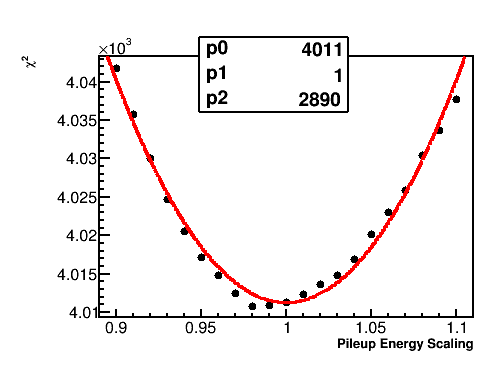
\includegraphics[width=\textwidth]{TMethod_Chi2_Vs_PileupEnergyScaling_Canv}
        \caption{T-Method \chisq versus pileup energy scale. The parabolic fit equation used was $y = p_{2}(x - p_{1})^{2} + p_{0}.$}
    \end{subfigure}% %you need this % here to add spacing between subfigures
    \hspace{1cm}
    \begin{subfigure}[t]{0.45\textwidth}
        \centering
        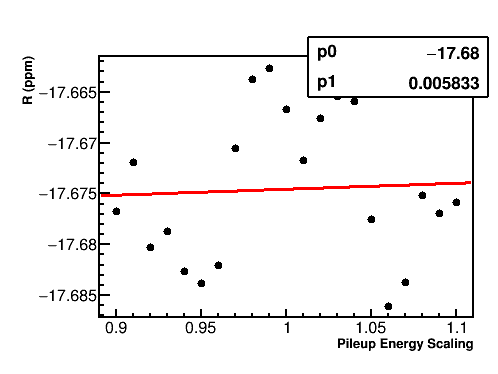
\includegraphics[width=\textwidth]{TMethod_R_Vs_PileupEnergyScaling_Canv}
        \caption{T-Method $R$ versus pileup energy scale. The parameter $p_{1}$ gives the sensitivity of $R$ to the value of the pileup energy scale, with units in ppm.}
    \end{subfigure}

    \begin{subfigure}[t]{0.45\textwidth}
        \centering
        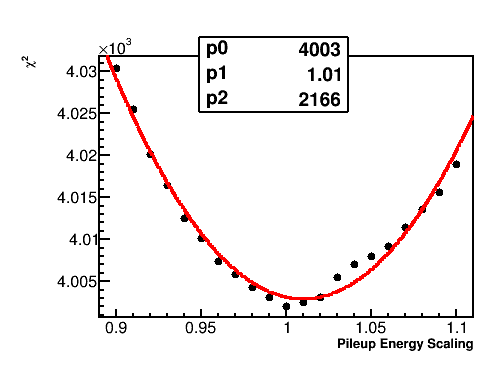
\includegraphics[width=\textwidth]{FullRatio_Chi2_Vs_PileupEnergyScaling_Canv}
        \caption{R-Method \chisq versus pileup energy scale. The parabolic fit equation used was $y = p_{2}(x - p_{1})^{2} + p_{0}.$}
    \end{subfigure}% %you need this % here to add spacing between subfigures
    \hspace{1cm}
    \begin{subfigure}[t]{0.45\textwidth}
        \centering
        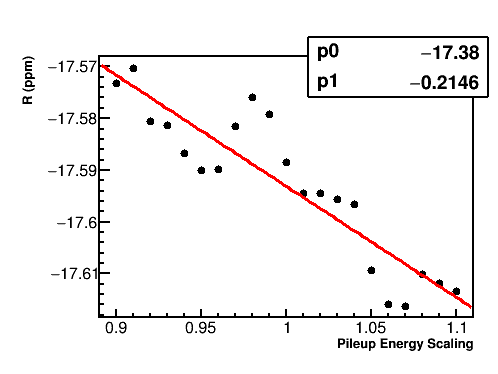
\includegraphics[width=\textwidth]{FullRatio_R_Vs_PileupEnergyScaling_Canv}
        \caption{R-Method $R$ versus pileup energy scale. The parameter $p_{1}$ gives the sensitivity of $R$ to the value of the pileup energy scale, with units in ppm.}
    \end{subfigure}
\caption[Pileup energy scale scan]{Pileup energy scale scan. Data are from the 9d dataset.}
\label{fig:PESscan}
\end{figure}



Since simulations however show that the energy resolution is much better than that determined by the \chisq, as shown in \figref{fig:ReconEastDoubletEnergyRatios}, and because of the non-linear slopes in some datasets, the uncertainty is instead taken as the max $\Delta R$ when applying a $\pm1\%$ scale factor on the doublet energy. This is only slightly conservative as the maximum ratio difference for energy sums larger than \SI{1.7}{\GeV} is about 1.1\%. Recon West is not expected to be significantly different, and the lack of spatial separation would imply that this ratio would be closer to 1, in the ballpark of 0.5\% or so. The systematic uncertainty is given in \tabref{tab:systematicError_clusterEnergyModel}.


\begin{figure}[h]
\centering
    \begin{subfigure}[t]{0.45\textwidth}
        \centering
        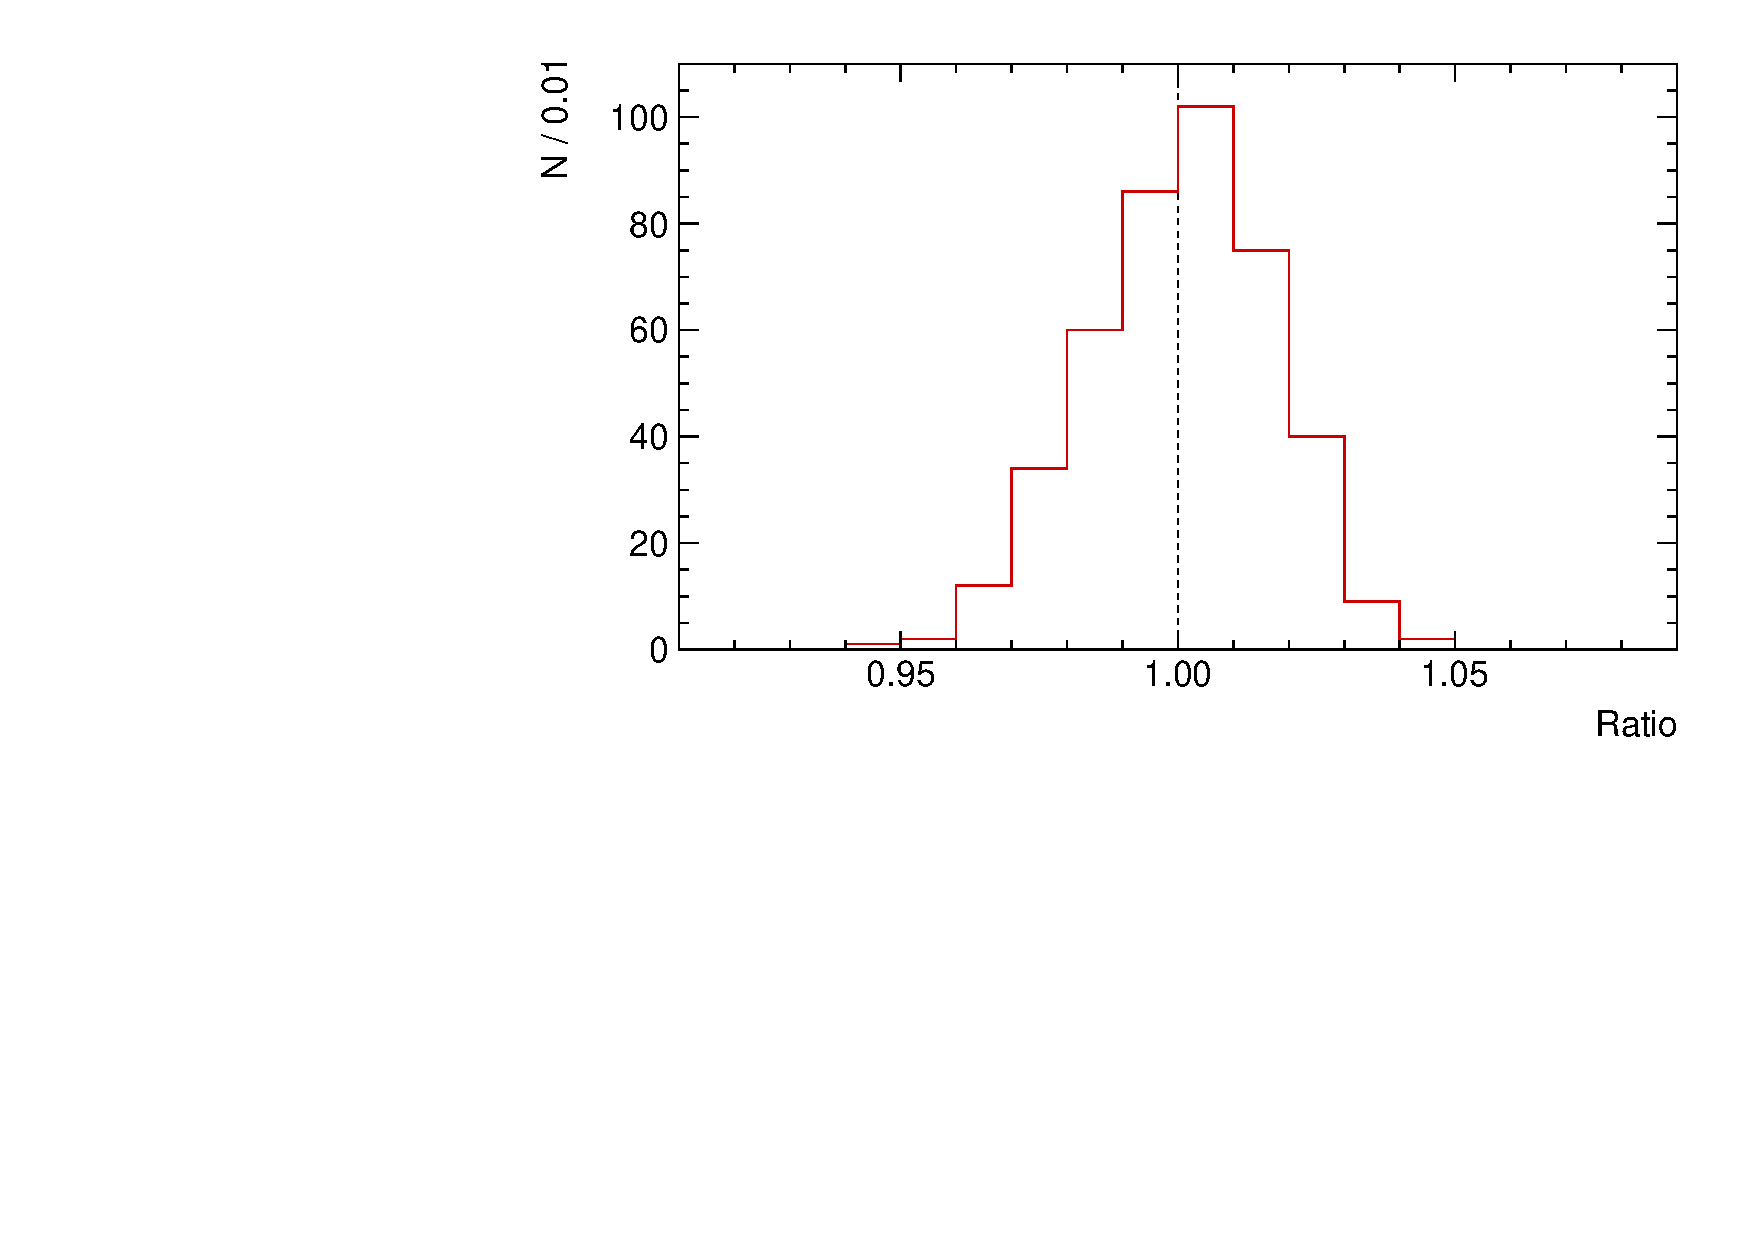
\includegraphics[width=\textwidth]{p_ratio_2_2_hist}
        \caption{The ratio of the doublet energy to the sum of the two singlets for two positrons of 2 \GeV.}
    \end{subfigure}%
    \hspace{1cm}
    \begin{subfigure}[t]{0.45\textwidth}
        \centering
        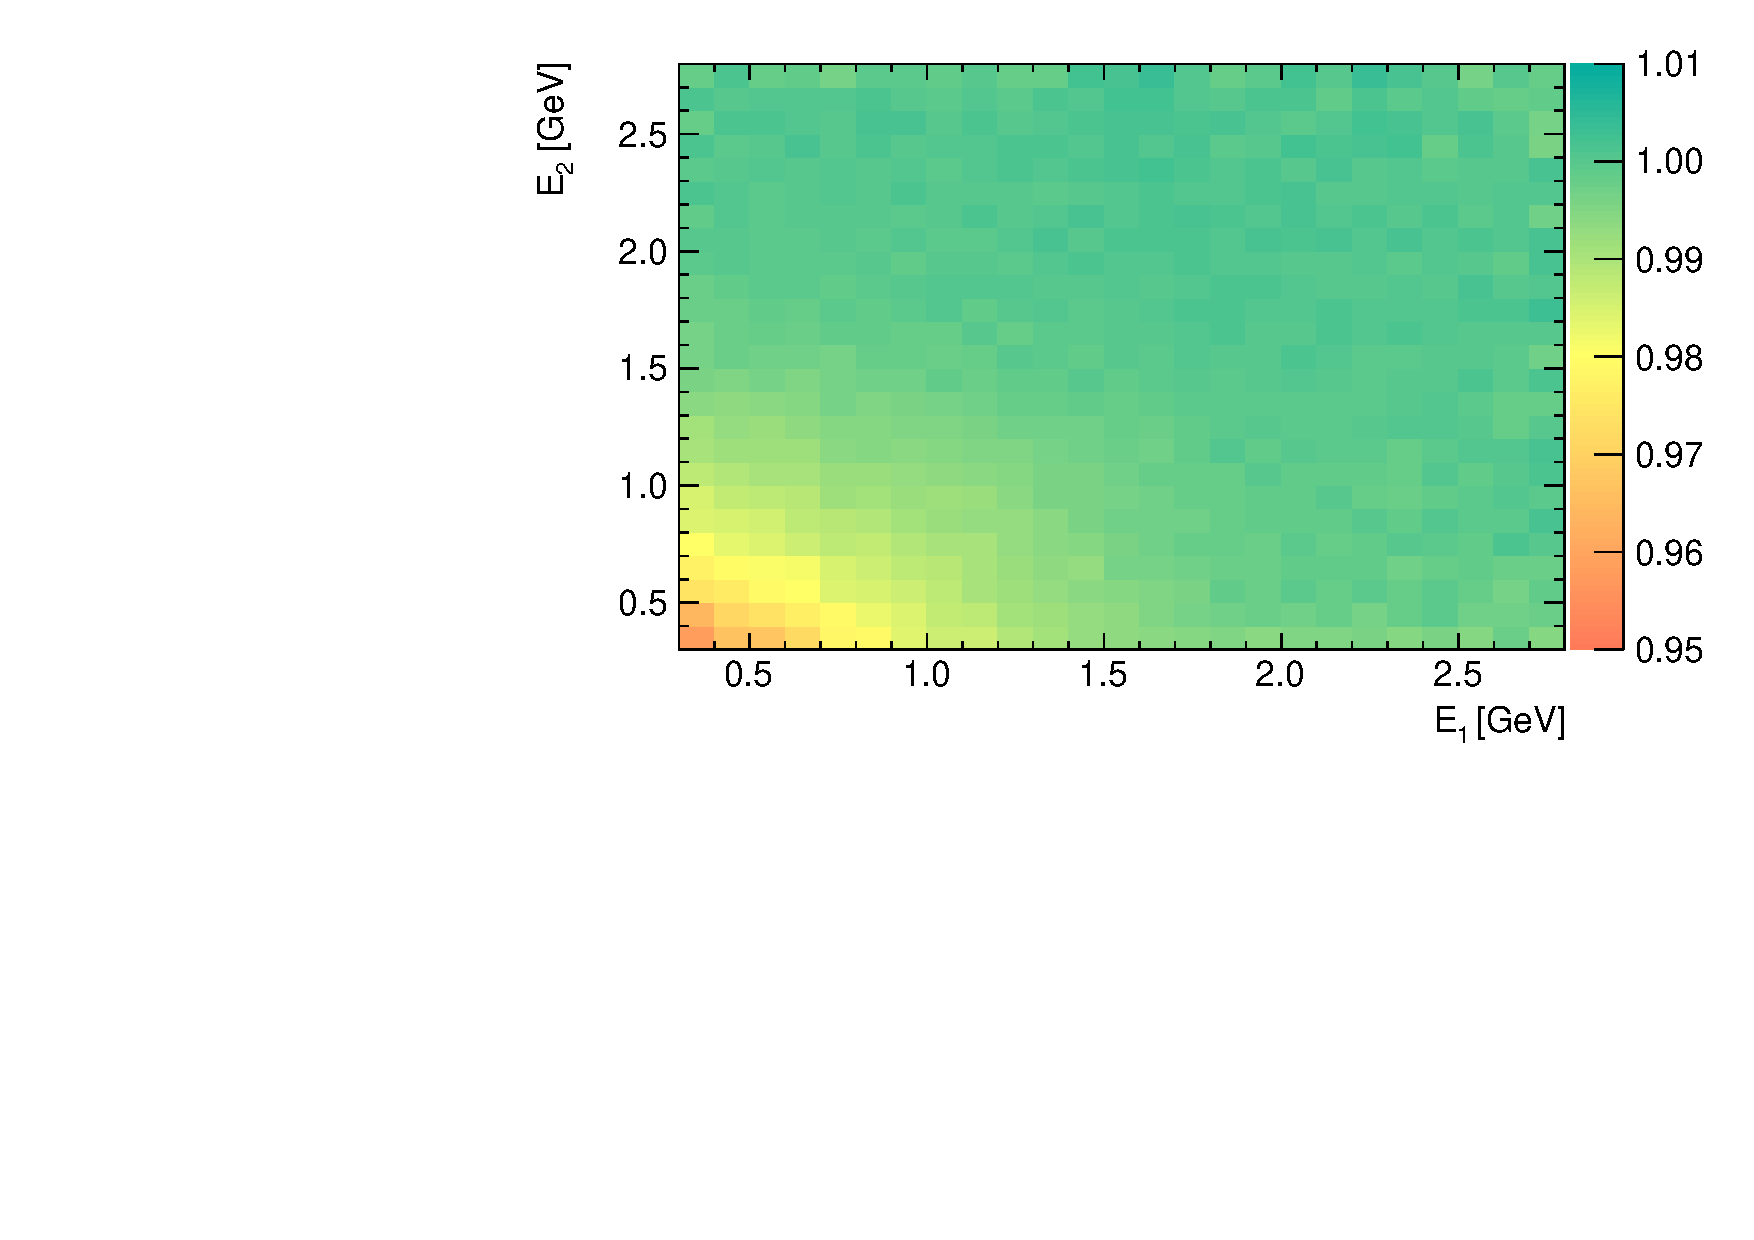
\includegraphics[width=\textwidth]{p_ratio_e1_e2}
        \caption{The average ratio of the doublet energy to the sum of the two singlets as a function of singlet energies.}
    \end{subfigure}
\caption[]{David fired two positrons at the calorimeter using MDC1 and for pileup cases calculated the ratio of the doublet energy to the two singlets. The plot on the left is for one set of energies, and the plot on the right is the average ratio. For low energies the energy can be quite a bit off, for energies above 1.7 \GeV it's more like 1\%. Plots courtesy of David Sweigart.}
\label{fig:ReconEastDoubletEnergyRatios}
\end{figure}


\begin{table}[h]
\centering
\renewcommand{\arraystretch}{1.2}
\begin{tabularx}{0.75\linewidth}{@{\extracolsep{\fill}}XYY}
  \hline
    \multicolumn{3}{c}{\textbf{Systematic Uncertainty due to Cluster Energy Model}} \\
  \hline\hline
    Dataset & \thead{T-Method} & \thead{R-Method} \\
  \hline
    60h & 11.0 & 10.9 \\
    HighKick & 4.8 & 7.2 \\
    9d & 6.1 & 10.2 \\ 
    Endgame & 10.0 & 6.8 \\
  \hline
\end{tabularx}
\caption[]{Systematic uncertainty due to cluster energy model. Units are in ppb.}
\label{tab:systematicError_clusterEnergyModel}
\end{table}




\clearpage
\subsection{Pileup Rate Uncertainty}

The pileup rate uncertainty arises from the fact that the pileup is estimated from pulses at times $t$ and $t+SGT$ and then placed at $t+SGT/2$. Ideally the pileup would have been estimated at those latter times from the beginning. There will be differences due to the muon precession and beam dynamics. Because my SGT is very small at \ns{10}, this uncertainty can be expected to be negligible. Using the prescription as outlined in David's thesis \cite{phdthesis:2020Sweigart}, I estimate the pileup rate uncertainty as 

\begin{align}
	\frac{N^{2}(t) - N(t-\frac{SGT}{2})N(t+\frac{SGT}{2})}{N^{2}(t)},
\end{align}
where $N(t)$ is the fit function determined from a T-Method fit to the data. $N^{2}(t)$ is what we wanted to use when constructing the pileup, but $N(t-\frac{SGT}{2})N(t+\frac{SGT}{2})$ is what we actually used. The rate uncertainty is shown in Figures~\ref{fig:pileupRateError} and \ref{fig:pileupRateErrorZoomed}.

There are some interesting features to point out. The pileup rate uncertainty oscillates at \wa and the shape is constant throughout the fill. The black points in the figure come from the nominal fit, where each graph point is calculated and spaced at 149.2/50 ns = 2.984 ns apart. It turns out that there are spikes at the boundaries of the points as defined in the fit function in ROOT. If I fit with 10x the number of points up to 100,000 as shown in the red graph points, the the spikes accordingly shift, and the shape appears to change. This is an effect of the discretization of the points in the ROOT function used to fit the data. The blue points show the average of the black points over a bin width, and as shown lie in line with the red points. Accounting for the discretization then by averaging over the bin width, the pileup rate uncertainty can be determined from the blue curve and is seen to only wander a maximum of 0.005\%, or 0.00005, away from 0. This is a negligible change in the rate, and the systematic uncertainty is thus taken to be 0 ppb for all datasets. Note that even if the maximum of the black curve were to be taken as the rate uncertainty, then it is still less than 0.04\% or 0.0004 and the systematic uncertainty would still be negligible.


\begin{figure}
    \centering
    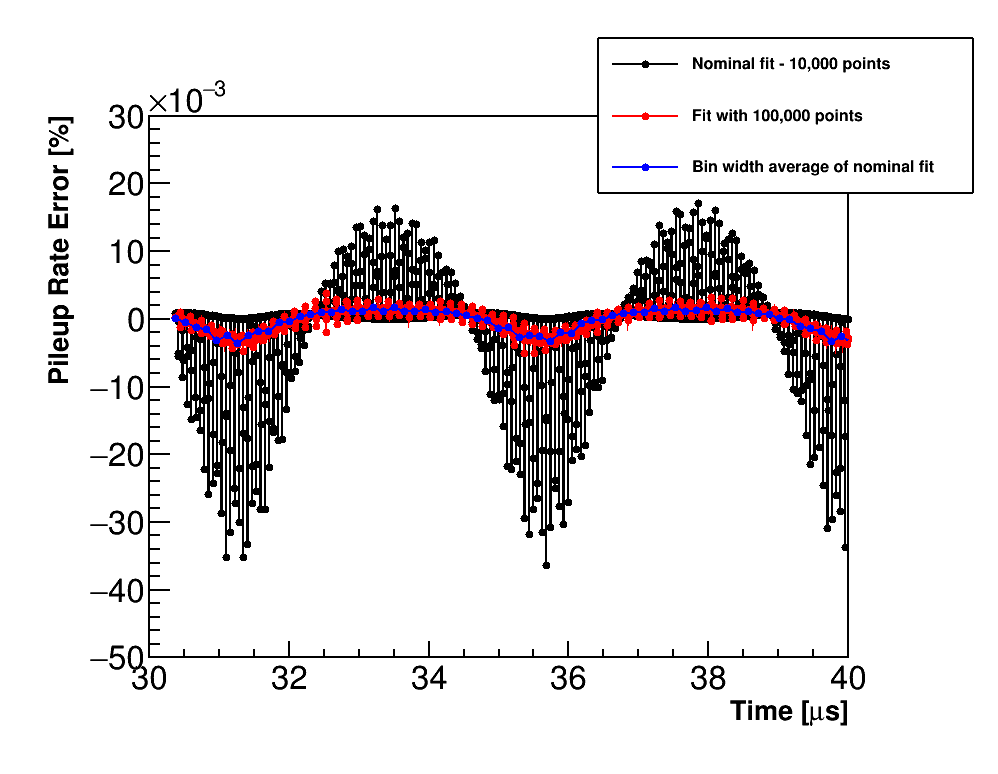
\includegraphics[width=.8\textwidth]{PileupRateError}
    \caption[]{Pileup rate uncertainty. Black points come from the nominal fit, which includes 10,000 points in the ROOT fit function. Red points come from a fit function with 100,000 points, and the blue points are the average of the black points over bin widths. Data are from the 60h dataset.}
    \label{fig:pileupRateError}
\end{figure}

\begin{figure}
    \centering
    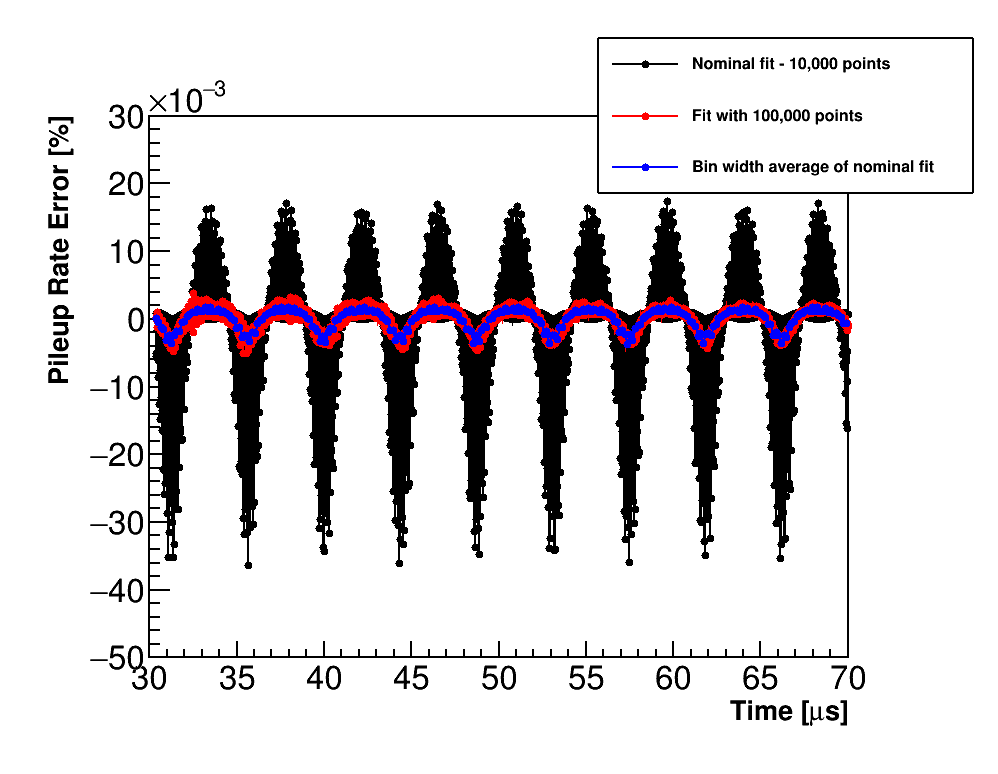
\includegraphics[width=.8\textwidth]{PileupRateError_ZoomedOut}
    \caption[]{The pileup rate uncertainty zoomed out, showing the consistency of the pileup rate uncertainty at later times in the fill. Data are from the 60h dataset.}
    \label{fig:pileupRateErrorZoomed}
\end{figure}

If instead a gap time of \SI{149.2}{\ns} were to be used, the the pileup rate uncertainty is significantly larger as shown in \figref{fig:pileupRateErrorLarger}, oscillating between -0.7\% and 0.3\%. This plot is comparable to David's thesis plot 6.28. Note that spikes can still be seen in the function however due to the discretization, though the relative size of them is much smaller than the rest of the curve.


\begin{figure}
    \centering
    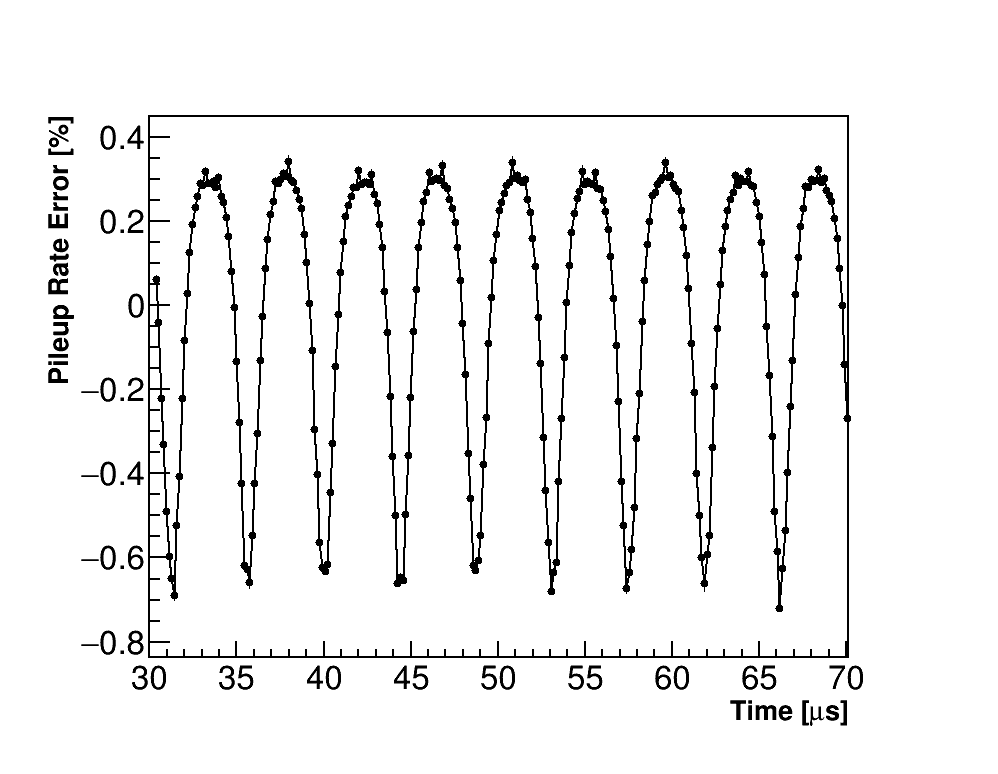
\includegraphics[width=.8\textwidth]{PileupRateError_149p2SGT}
    \caption[]{Pileup rate uncertainty when using a gap time of \SI{149.2}{\ns}. Data are from the 60h dataset.}
    \label{fig:pileupRateErrorLarger}
\end{figure}




\clearpage
\subsection{Unseen Pileup}

The systematic uncertainty due to unseen pileup is given in \tabref{tab:systematicError_unseenPileup}. They are calculated by ignoring pileup pulses below \SI{100}{\MeV} in the pileup construction, a value which twice as high as the expected missed pulse energies of around \SI{50}{\MeV} or less. If the threshold is raised to \SI{200}{\MeV} then the systematic uncertainties range around in the ballpark from 10-30 ppb.

\begin{table}
\centering
\renewcommand{\arraystretch}{1.2}
\begin{tabularx}{0.65\linewidth}{@{\extracolsep{\fill}}XYY}
  \hline
    \multicolumn{3}{c}{\textbf{Systematic Uncertainty due to Unseen Pileup}} \\
  \hline\hline
    Dataset & \thead{T-Method} & \thead{R-Method} \\
  \hline
    60h & 0.8 & 0.6 \\
    HighKick & 1.3 & 0.1 \\
    9d & 2.5 & 2.5 \\ 
    Endgame & 4.1 & 2.4 \\
  \hline
\end{tabularx}
\caption[]{Systematic uncertainty due to unseen pileup. Units are in ppb.}
\label{tab:systematicError_unseenPileup}
\end{table}



\clearpage
\subsection{Triple Pileup Correction}

Triple pileup is not included in my pileup correction. The systematic uncertainty for ignoring the triples is estimated by looking at the $\Delta R$ with and without the doubles correction (which can be gotten from the slopes of the pileup multiplier scans extrapolated to 0, \tabref{tab:pileupMultplierScan}), multiplied against the rate of triples to doubles. The latter can be approximated by the rate of doubles to singles, a plot of which is given in \figref{fig:pileupRateFraction}. As shown the fraction of the pileup is less than 1\% and decreases throughout the fill. The rate is averaged over the first \gmtwo period in the fit before multiplying against the $\Delta R$, the values are given in \tabref{tab:pileupRates}. The systematic uncertainties are given in \tabref{tab:systematicError_triplePileupCorrection}. Even these small numbers here are conservative since the rate drops throughout the fill, and would drop even faster for triples to doubles.


\begin{figure}[h]
    \centering
    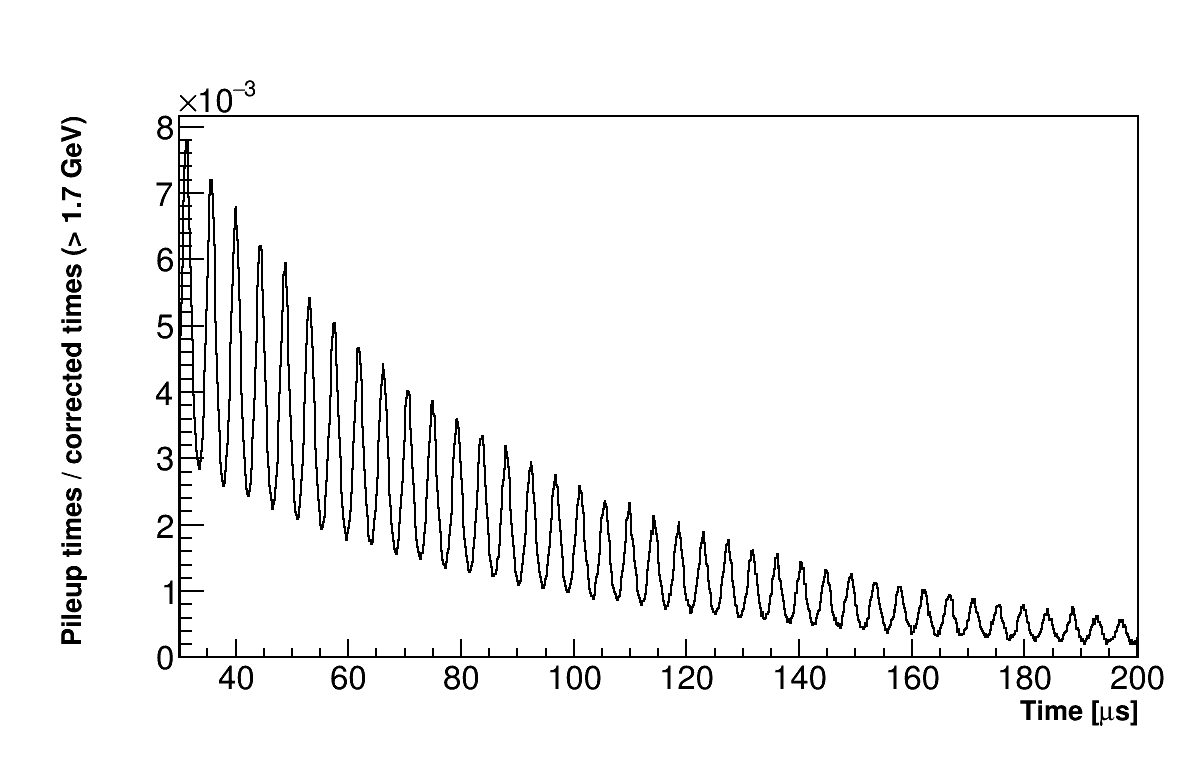
\includegraphics[width=1\textwidth]{pileupRateFraction}
    \caption[]{Pileup rate fraction plot. Data from the Endgame dataset.}
    \label{fig:pileupRateFraction}
\end{figure}


\begin{table}[h]
\centering
\renewcommand{\arraystretch}{1.2}
\begin{tabularx}{0.65\linewidth}{@{\extracolsep{\fill}}lcc}
  \hline
    \multicolumn{3}{c}{\textbf{Pileup Rates}} \\
  \hline\hline
    Dataset & Average rate & Max rate \\
  \hline
    60h & \num{5.33e-3} & \num{8.50e-3} \\
    HighKick & \num{5.69e-3} & \num{8.96e-3} \\
    9d & \num{5.19e-3} & \num{8.32e-3} \\ 
    Endgame & \num{4.93e-3} & \num{7.78e-3} \\
  \hline
\end{tabularx}
\caption[]{Pileup rates over the first \gmtwo period of the fitting range, averaged and the maximum value respectively.}
\label{tab:pileupRates}
\end{table}


\begin{table}[h]
\centering
\renewcommand{\arraystretch}{1.2}
\begin{tabularx}{0.75\linewidth}{@{\extracolsep{\fill}}XYY}
  \hline
    \multicolumn{3}{c}{\textbf{Systematic Uncertainty due to Triple Pileup Correction}} \\
  \hline\hline
    Dataset & \thead{T-Method} & \thead{R-Method} \\
  \hline
    60h & 1.9 & 1.6 \\
    HighKick & 1.3 & 1.2 \\
    9d & 1.0 & 1.1 \\ 
    Endgame & 1.6 & 1.3 \\
  \hline
\end{tabularx}
\caption[]{Systematic uncertainty due to triple pileup correction. Units are in ppb.}
\label{tab:systematicError_triplePileupCorrection}
\end{table}



